\documentclass[1p]{elsarticle_modified}
%\bibliographystyle{elsarticle-num}

%\usepackage[colorlinks]{hyperref}
%\usepackage{abbrmath_seonhwa} %\Abb, \Ascr, \Acal ,\Abf, \Afrak
\usepackage{amsfonts}
\usepackage{amssymb}
\usepackage{amsmath}
\usepackage{amsthm}
\usepackage{scalefnt}
\usepackage{amsbsy}
\usepackage{kotex}
\usepackage{caption}
\usepackage{subfig}
\usepackage{color}
\usepackage{graphicx}
\usepackage{xcolor} %% white, black, red, green, blue, cyan, magenta, yellow
\usepackage{float}
\usepackage{setspace}
\usepackage{hyperref}

\usepackage{tikz}
\usetikzlibrary{arrows}

\usepackage{multirow}
\usepackage{array} % fixed length table
\usepackage{hhline}

%%%%%%%%%%%%%%%%%%%%%
\makeatletter
\renewcommand*\env@matrix[1][\arraystretch]{%
	\edef\arraystretch{#1}%
	\hskip -\arraycolsep
	\let\@ifnextchar\new@ifnextchar
	\array{*\c@MaxMatrixCols c}}
\makeatother %https://tex.stackexchange.com/questions/14071/how-can-i-increase-the-line-spacing-in-a-matrix
%%%%%%%%%%%%%%%

\usepackage[normalem]{ulem}

\newcommand{\msout}[1]{\ifmmode\text{\sout{\ensuremath{#1}}}\else\sout{#1}\fi}
%SOURCE: \msout is \stkout macro in https://tex.stackexchange.com/questions/20609/strikeout-in-math-mode

\newcommand{\cancel}[1]{
	\ifmmode
	{\color{red}\msout{#1}}
	\else
	{\color{red}\sout{#1}}
	\fi
}

\newcommand{\add}[1]{
	{\color{blue}\uwave{#1}}
}

\newcommand{\replace}[2]{
	\ifmmode
	{\color{red}\msout{#1}}{\color{blue}\uwave{#2}}
	\else
	{\color{red}\sout{#1}}{\color{blue}\uwave{#2}}
	\fi
}

\newcommand{\Sol}{\mathcal{S}} %segment
\newcommand{\D}{D} %diagram
\newcommand{\A}{\mathcal{A}} %arc


%%%%%%%%%%%%%%%%%%%%%%%%%%%%%5 test

\def\sl{\operatorname{\textup{SL}}(2,\Cbb)}
\def\psl{\operatorname{\textup{PSL}}(2,\Cbb)}
\def\quan{\mkern 1mu \triangleright \mkern 1mu}

\theoremstyle{definition}
\newtheorem{thm}{Theorem}[section]
\newtheorem{prop}[thm]{Proposition}
\newtheorem{lem}[thm]{Lemma}
\newtheorem{ques}[thm]{Question}
\newtheorem{cor}[thm]{Corollary}
\newtheorem{defn}[thm]{Definition}
\newtheorem{exam}[thm]{Example}
\newtheorem{rmk}[thm]{Remark}
\newtheorem{alg}[thm]{Algorithm}

\newcommand{\I}{\sqrt{-1}}
\begin{document}

%\begin{frontmatter}
%
%\title{Boundary parabolic representations of knots up to 8 crossings}
%
%%% Group authors per affiliation:
%\author{Yunhi Cho} 
%\address{Department of Mathematics, University of Seoul, Seoul, Korea}
%\ead{yhcho@uos.ac.kr}
%
%
%\author{Seonhwa Kim} %\fnref{s_kim}}
%\address{Center for Geometry and Physics, Institute for Basic Science, Pohang, 37673, Korea}
%\ead{ryeona17@ibs.re.kr}
%
%\author{Hyuk Kim}
%\address{Department of Mathematical Sciences, Seoul National University, Seoul 08826, Korea}
%\ead{hyukkim@snu.ac.kr}
%
%\author{Seokbeom Yoon}
%\address{Department of Mathematical Sciences, Seoul National University, Seoul, 08826,  Korea}
%\ead{sbyoon15@snu.ac.kr}
%
%\begin{abstract}
%We find all boundary parabolic representation of knots up to 8 crossings.
%
%\end{abstract}
%\begin{keyword}
%    \MSC[2010] 57M25 
%\end{keyword}
%
%\end{frontmatter}

%\linenumbers
%\tableofcontents
%
\newcommand\colored[1]{\textcolor{white}{\rule[-0.35ex]{0.8em}{1.4ex}}\kern-0.8em\color{red} #1}%
%\newcommand\colored[1]{\textcolor{white}{ #1}\kern-2.17ex	\textcolor{white}{ #1}\kern-1.81ex	\textcolor{white}{ #1}\kern-2.15ex\color{red}#1	}

{\Large $\underline{12a_{1034}~(K12a_{1034})}$}

\setlength{\tabcolsep}{10pt}
\renewcommand{\arraystretch}{1.6}
\vspace{1cm}\begin{tabular}{m{100pt}>{\centering\arraybackslash}m{274pt}}
\multirow{5}{120pt}{
	\centering
	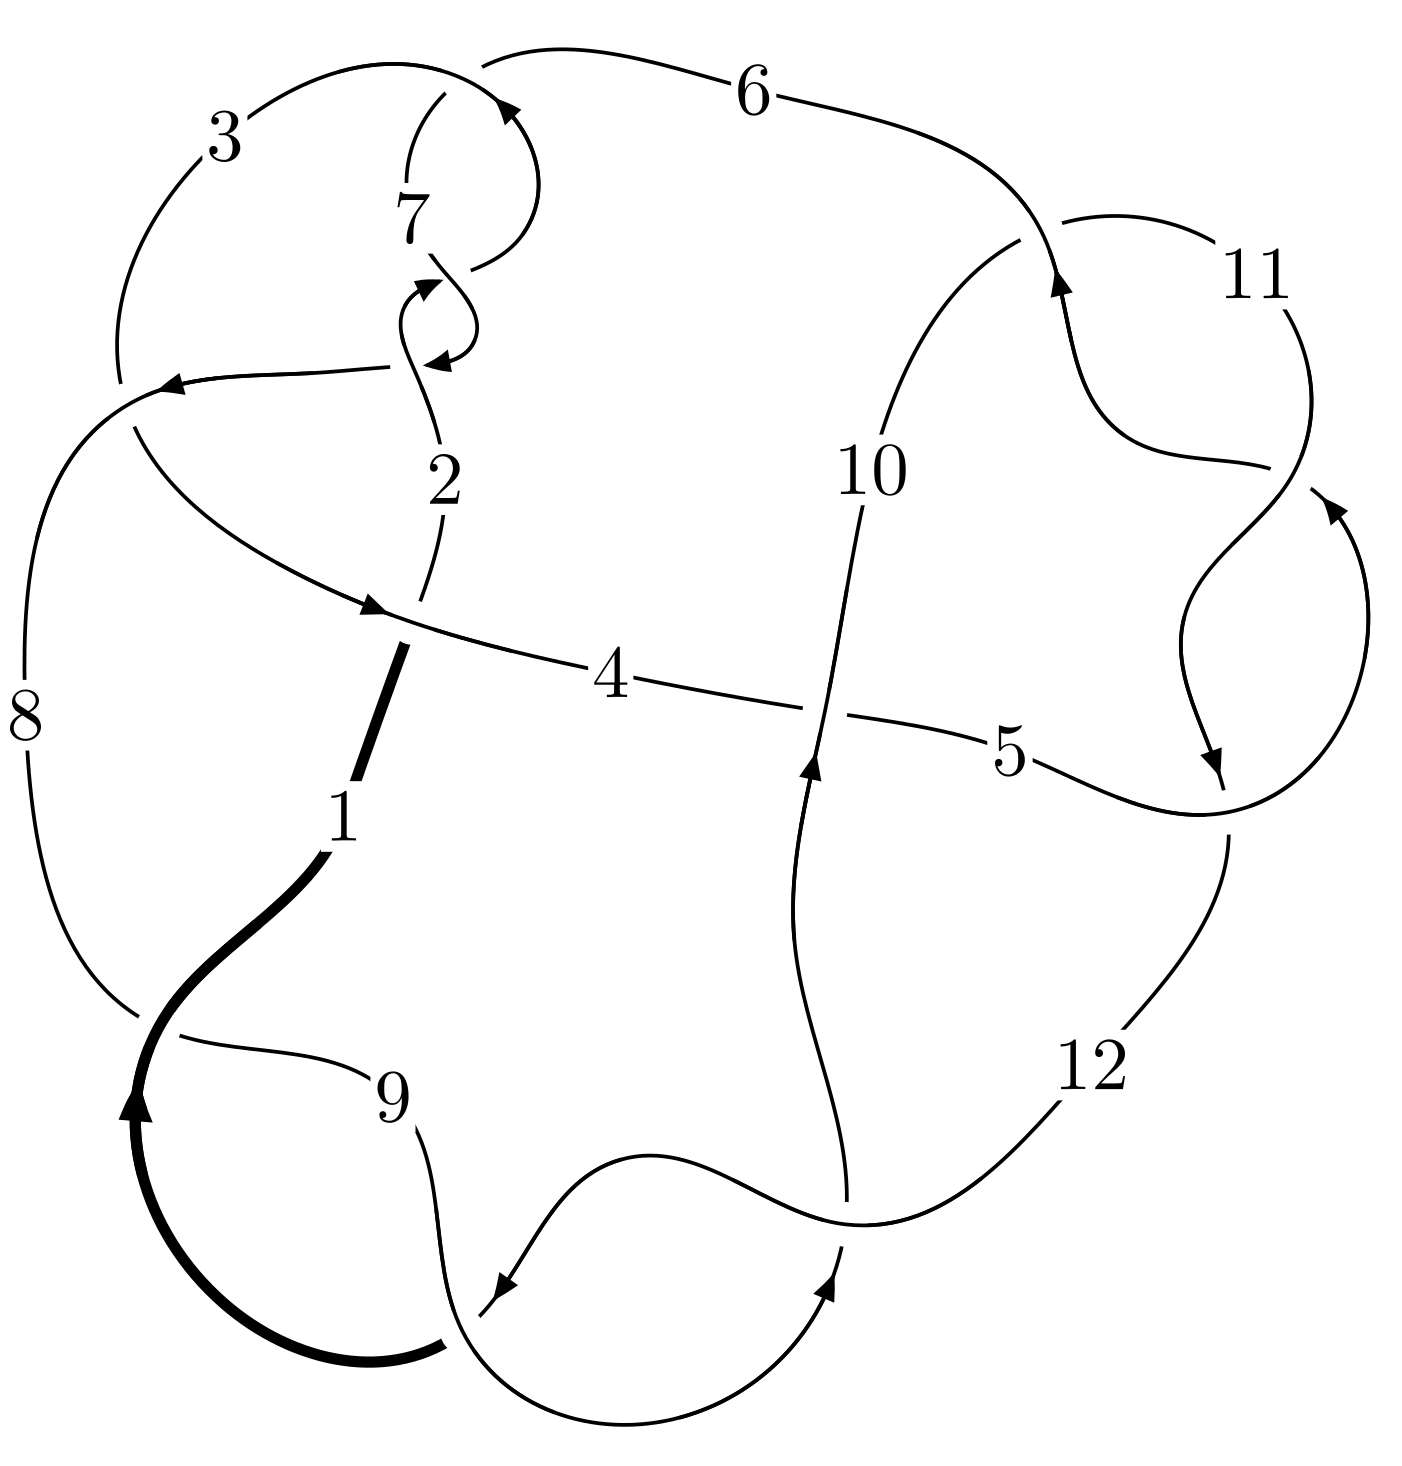
\includegraphics[width=112pt]{../../../GIT/diagram.site/Diagrams/png/1835_12a_1034.png}\\
\ \ \ A knot diagram\footnotemark}&
\allowdisplaybreaks
\textbf{Linearized knot diagam} \\
\cline{2-2}
 &
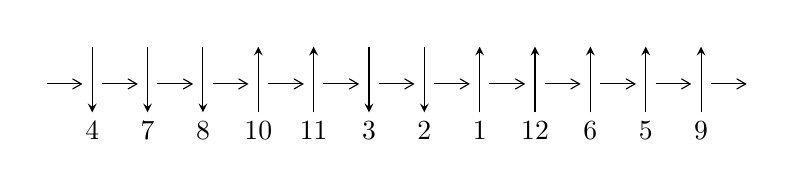
\begin{tikzpicture}[x=20pt, y=17pt]
	% nodes
	\node (C0) at (0, 0) {};
	\node (C1) at (1, 0) {};
	\node (C1U) at (1, +1) {};
	\node (C1D) at (1, -1) {4};

	\node (C2) at (2, 0) {};
	\node (C2U) at (2, +1) {};
	\node (C2D) at (2, -1) {7};

	\node (C3) at (3, 0) {};
	\node (C3U) at (3, +1) {};
	\node (C3D) at (3, -1) {8};

	\node (C4) at (4, 0) {};
	\node (C4U) at (4, +1) {};
	\node (C4D) at (4, -1) {10};

	\node (C5) at (5, 0) {};
	\node (C5U) at (5, +1) {};
	\node (C5D) at (5, -1) {11};

	\node (C6) at (6, 0) {};
	\node (C6U) at (6, +1) {};
	\node (C6D) at (6, -1) {3};

	\node (C7) at (7, 0) {};
	\node (C7U) at (7, +1) {};
	\node (C7D) at (7, -1) {2};

	\node (C8) at (8, 0) {};
	\node (C8U) at (8, +1) {};
	\node (C8D) at (8, -1) {1};

	\node (C9) at (9, 0) {};
	\node (C9U) at (9, +1) {};
	\node (C9D) at (9, -1) {12};

	\node (C10) at (10, 0) {};
	\node (C10U) at (10, +1) {};
	\node (C10D) at (10, -1) {6};

	\node (C11) at (11, 0) {};
	\node (C11U) at (11, +1) {};
	\node (C11D) at (11, -1) {5};

	\node (C12) at (12, 0) {};
	\node (C12U) at (12, +1) {};
	\node (C12D) at (12, -1) {9};
	\node (C13) at (13, 0) {};

	% arrows
	\draw[->,>={angle 60}]
	(C0) edge (C1) (C1) edge (C2) (C2) edge (C3) (C3) edge (C4) (C4) edge (C5) (C5) edge (C6) (C6) edge (C7) (C7) edge (C8) (C8) edge (C9) (C9) edge (C10) (C10) edge (C11) (C11) edge (C12) (C12) edge (C13) ;	\draw[->,>=stealth]
	(C1U) edge (C1D) (C2U) edge (C2D) (C3U) edge (C3D) (C4D) edge (C4U) (C5D) edge (C5U) (C6U) edge (C6D) (C7U) edge (C7D) (C8D) edge (C8U) (C9D) edge (C9U) (C10D) edge (C10U) (C11D) edge (C11U) (C12D) edge (C12U) ;
	\end{tikzpicture} \\
\hhline{~~} \\& 
\textbf{Solving Sequence} \\ \cline{2-2} 
 &
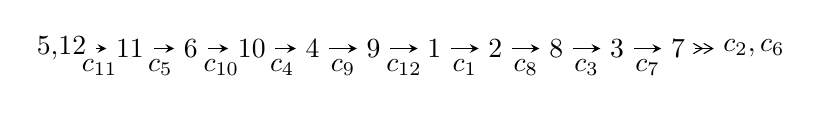
\begin{tikzpicture}[x=22pt, y=7pt]
	% node
	\node (A0) at (-1/8, 0) {5,12};
	\node (A1) at (1, 0) {11};
	\node (A2) at (2, 0) {6};
	\node (A3) at (3, 0) {10};
	\node (A4) at (4, 0) {4};
	\node (A5) at (5, 0) {9};
	\node (A6) at (6, 0) {1};
	\node (A7) at (7, 0) {2};
	\node (A8) at (8, 0) {8};
	\node (A9) at (9, 0) {3};
	\node (A10) at (10, 0) {7};
	\node (C1) at (1/2, -1) {$c_{11}$};
	\node (C2) at (3/2, -1) {$c_{5}$};
	\node (C3) at (5/2, -1) {$c_{10}$};
	\node (C4) at (7/2, -1) {$c_{4}$};
	\node (C5) at (9/2, -1) {$c_{9}$};
	\node (C6) at (11/2, -1) {$c_{12}$};
	\node (C7) at (13/2, -1) {$c_{1}$};
	\node (C8) at (15/2, -1) {$c_{8}$};
	\node (C9) at (17/2, -1) {$c_{3}$};
	\node (C10) at (19/2, -1) {$c_{7}$};
	\node (A11) at (45/4, 0) {$c_{2},c_{6}$};

	% edge
	\draw[->,>=stealth]	
	(A0) edge (A1) (A1) edge (A2) (A2) edge (A3) (A3) edge (A4) (A4) edge (A5) (A5) edge (A6) (A6) edge (A7) (A7) edge (A8) (A8) edge (A9) (A9) edge (A10) ;
	\draw[->>,>={angle 60}]	
	(A10) edge (A11);
\end{tikzpicture} \\ 

\end{tabular} \\

\footnotetext{
The image of knot diagram is generated by the software ``\textbf{Draw programme}" developed by Andrew Bartholomew(\url{http://www.layer8.co.uk/maths/draw/index.htm\#Running-draw}), where we modified some parts for our purpose(\url{https://github.com/CATsTAILs/LinksPainter}).
}\phantom \\ \newline 
\centering \textbf{Ideals for irreducible components\footnotemark of $X_{\text{par}}$} 
 
\begin{align*}
I^u_{1}&=\langle 
u^{60}+u^{59}+\cdots- u^2+1\rangle \\
\\
\end{align*}
\raggedright * 1 irreducible components of $\dim_{\mathbb{C}}=0$, with total 60 representations.\\
\footnotetext{All coefficients of polynomials are rational numbers. But the coefficients are sometimes approximated in decimal forms when there is not enough margin.}
\newpage
\renewcommand{\arraystretch}{1}
\centering \section*{I. $I^u_{1}= \langle u^{60}+u^{59}+\cdots- u^2+1 \rangle$}
\flushleft \textbf{(i) Arc colorings}\\
\begin{tabular}{m{7pt} m{180pt} m{7pt} m{180pt} }
\flushright $a_{5}=$&$\begin{pmatrix}0\\u\end{pmatrix}$ \\
\flushright $a_{12}=$&$\begin{pmatrix}1\\0\end{pmatrix}$ \\
\flushright $a_{11}=$&$\begin{pmatrix}1\\u^2\end{pmatrix}$ \\
\flushright $a_{6}=$&$\begin{pmatrix}u\\u^3+u\end{pmatrix}$ \\
\flushright $a_{10}=$&$\begin{pmatrix}u^2+1\\u^4+2 u^2\end{pmatrix}$ \\
\flushright $a_{4}=$&$\begin{pmatrix}- u^5-2 u^3- u\\- u^7-3 u^5-2 u^3+u\end{pmatrix}$ \\
\flushright $a_{9}=$&$\begin{pmatrix}- u^4- u^2+1\\u^4+2 u^2\end{pmatrix}$ \\
\flushright $a_{1}=$&$\begin{pmatrix}u^8+3 u^6+u^4-2 u^2+1\\- u^8-4 u^6-4 u^4\end{pmatrix}$ \\
\flushright $a_{2}=$&$\begin{pmatrix}u^{20}+9 u^{18}+\cdots-3 u^2+1\\u^{22}+10 u^{20}+\cdots-10 u^4+u^2\end{pmatrix}$ \\
\flushright $a_{8}=$&$\begin{pmatrix}- u^{12}-5 u^{10}-7 u^8+2 u^4-3 u^2+1\\u^{12}+6 u^{10}+12 u^8+8 u^6+u^4+2 u^2\end{pmatrix}$ \\
\flushright $a_{3}=$&$\begin{pmatrix}- u^{31}-14 u^{29}+\cdots+20 u^5-8 u^3\\u^{31}+15 u^{29}+\cdots-8 u^5+u\end{pmatrix}$ \\
\flushright $a_{7}=$&$\begin{pmatrix}u^{54}+25 u^{52}+\cdots-2 u^2+1\\u^{56}+26 u^{54}+\cdots+2 u^4+2 u^2\end{pmatrix}$\\&\end{tabular}
\flushleft \textbf{(ii) Obstruction class $= -1$}\\~\\
\flushleft \textbf{(iii) Cusp Shapes $= -4 u^{58}-4 u^{57}+\cdots+4 u+2$}\\~\\
\newpage\renewcommand{\arraystretch}{1}
\flushleft \textbf{(iv) u-Polynomials at the component}\newline \\
\begin{tabular}{m{50pt}|m{274pt}}
Crossings & \hspace{64pt}u-Polynomials at each crossing \\
\hline $$\begin{aligned}c_{1}\end{aligned}$$&$\begin{aligned}
&u^{60}-15 u^{59}+\cdots-16 u+1
\end{aligned}$\\
\hline $$\begin{aligned}c_{2},c_{6},c_{7}\end{aligned}$$&$\begin{aligned}
&u^{60}+u^{59}+\cdots+2 u+1
\end{aligned}$\\
\hline $$\begin{aligned}c_{3}\end{aligned}$$&$\begin{aligned}
&u^{60}- u^{59}+\cdots+12 u+5
\end{aligned}$\\
\hline $$\begin{aligned}c_{4}\end{aligned}$$&$\begin{aligned}
&u^{60}- u^{59}+\cdots-976 u+457
\end{aligned}$\\
\hline $$\begin{aligned}c_{5},c_{10},c_{11}\end{aligned}$$&$\begin{aligned}
&u^{60}+u^{59}+\cdots- u^2+1
\end{aligned}$\\
\hline $$\begin{aligned}c_{8},c_{9},c_{12}\end{aligned}$$&$\begin{aligned}
&u^{60}+7 u^{59}+\cdots+176 u+17
\end{aligned}$\\
\hline
\end{tabular}\\~\\
\newpage\renewcommand{\arraystretch}{1}
\flushleft \textbf{(v) Riley Polynomials at the component}\newline \\
\begin{tabular}{m{50pt}|m{274pt}}
Crossings & \hspace{64pt}Riley Polynomials at each crossing \\
\hline $$\begin{aligned}c_{1}\end{aligned}$$&$\begin{aligned}
&y^{60}+y^{59}+\cdots+126 y+1
\end{aligned}$\\
\hline $$\begin{aligned}c_{2},c_{6},c_{7}\end{aligned}$$&$\begin{aligned}
&y^{60}+53 y^{59}+\cdots-2 y+1
\end{aligned}$\\
\hline $$\begin{aligned}c_{3}\end{aligned}$$&$\begin{aligned}
&y^{60}-7 y^{59}+\cdots+266 y+25
\end{aligned}$\\
\hline $$\begin{aligned}c_{4}\end{aligned}$$&$\begin{aligned}
&y^{60}+29 y^{59}+\cdots+6707658 y+208849
\end{aligned}$\\
\hline $$\begin{aligned}c_{5},c_{10},c_{11}\end{aligned}$$&$\begin{aligned}
&y^{60}+57 y^{59}+\cdots-2 y+1
\end{aligned}$\\
\hline $$\begin{aligned}c_{8},c_{9},c_{12}\end{aligned}$$&$\begin{aligned}
&y^{60}+65 y^{59}+\cdots+8430 y+289
\end{aligned}$\\
\hline
\end{tabular}\\~\\
\newpage\flushleft \textbf{(vi) Complex Volumes and Cusp Shapes}
$$\begin{array}{c|c|c}  
\text{Solutions to }I^u_{1}& \I (\text{vol} + \sqrt{-1}CS) & \text{Cusp shape}\\
 \hline 
\begin{aligned}
u &= -0.073972 + 1.163980 I\end{aligned}
 & \phantom{-}3.44486 - 4.07290 I & \phantom{-0.000000 } 0 \\ \hline\begin{aligned}
u &= -0.073972 - 1.163980 I\end{aligned}
 & \phantom{-}3.44486 + 4.07290 I & \phantom{-0.000000 } 0 \\ \hline\begin{aligned}
u &= -0.687972 + 0.447740 I\end{aligned}
 & -1.97103 - 10.12300 I & \phantom{-}1.79388 + 7.77303 I \\ \hline\begin{aligned}
u &= -0.687972 - 0.447740 I\end{aligned}
 & -1.97103 + 10.12300 I & \phantom{-}1.79388 - 7.77303 I \\ \hline\begin{aligned}
u &= \phantom{-}0.680583 + 0.456074 I\end{aligned}
 & -7.13842 + 6.32141 I & -2.86224 - 6.81848 I \\ \hline\begin{aligned}
u &= \phantom{-}0.680583 - 0.456074 I\end{aligned}
 & -7.13842 - 6.32141 I & -2.86224 + 6.81848 I \\ \hline\begin{aligned}
u &= -0.634060 + 0.514914 I\end{aligned}
 & -2.22403 + 5.72401 I & \phantom{-}1.08593 - 1.85120 I \\ \hline\begin{aligned}
u &= -0.634060 - 0.514914 I\end{aligned}
 & -2.22403 - 5.72401 I & \phantom{-}1.08593 + 1.85120 I \\ \hline\begin{aligned}
u &= \phantom{-}0.642018 + 0.503673 I\end{aligned}
 & -7.31878 - 1.92743 I & -3.47550 + 0.73718 I \\ \hline\begin{aligned}
u &= \phantom{-}0.642018 - 0.503673 I\end{aligned}
 & -7.31878 + 1.92743 I & -3.47550 - 0.73718 I \\ \hline\begin{aligned}
u &= -0.664857 + 0.466839 I\end{aligned}
 & -5.12792 - 2.35466 I & -0.20423 + 2.11201 I \\ \hline\begin{aligned}
u &= -0.664857 - 0.466839 I\end{aligned}
 & -5.12792 + 2.35466 I & -0.20423 - 2.11201 I \\ \hline\begin{aligned}
u &= -0.651503 + 0.484423 I\end{aligned}
 & -5.19301 - 2.00819 I & -0.45901 + 4.03609 I \\ \hline\begin{aligned}
u &= -0.651503 - 0.484423 I\end{aligned}
 & -5.19301 + 2.00819 I & -0.45901 - 4.03609 I \\ \hline\begin{aligned}
u &= \phantom{-}0.042814 + 1.220540 I\end{aligned}
 & -1.97107 + 1.50217 I & \phantom{-0.000000 } 0 \\ \hline\begin{aligned}
u &= \phantom{-}0.042814 - 1.220540 I\end{aligned}
 & -1.97107 - 1.50217 I & \phantom{-0.000000 } 0 \\ \hline\begin{aligned}
u &= \phantom{-}0.624478 + 0.433571 I\end{aligned}
 & \phantom{-}1.64938 + 2.01589 I & \phantom{-}4.08259 - 3.48102 I \\ \hline\begin{aligned}
u &= \phantom{-}0.624478 - 0.433571 I\end{aligned}
 & \phantom{-}1.64938 - 2.01589 I & \phantom{-}4.08259 + 3.48102 I \\ \hline\begin{aligned}
u &= -0.181617 + 1.297260 I\end{aligned}
 & \phantom{-}2.13974 - 1.34166 I & \phantom{-0.000000 } 0 \\ \hline\begin{aligned}
u &= -0.181617 - 1.297260 I\end{aligned}
 & \phantom{-}2.13974 + 1.34166 I & \phantom{-0.000000 } 0 \\ \hline\begin{aligned}
u &= \phantom{-}0.614989 + 0.200876 I\end{aligned}
 & \phantom{-}5.34028 + 6.50684 I & \phantom{-}7.37974 - 8.13021 I \\ \hline\begin{aligned}
u &= \phantom{-}0.614989 - 0.200876 I\end{aligned}
 & \phantom{-}5.34028 - 6.50684 I & \phantom{-}7.37974 + 8.13021 I \\ \hline\begin{aligned}
u &= \phantom{-}0.163827 + 1.347560 I\end{aligned}
 & -3.62256 + 2.89228 I & \phantom{-0.000000 } 0 \\ \hline\begin{aligned}
u &= \phantom{-}0.163827 - 1.347560 I\end{aligned}
 & -3.62256 - 2.89228 I & \phantom{-0.000000 } 0 \\ \hline\begin{aligned}
u &= \phantom{-}0.219969 + 1.352410 I\end{aligned}
 & \phantom{-}0.44892 + 9.53691 I & \phantom{-0.000000 } 0 \\ \hline\begin{aligned}
u &= \phantom{-}0.219969 - 1.352410 I\end{aligned}
 & \phantom{-}0.44892 - 9.53691 I & \phantom{-0.000000 } 0 \\ \hline\begin{aligned}
u &= -0.202204 + 1.360380 I\end{aligned}
 & -4.85892 - 6.22848 I & \phantom{-0.000000 } 0 \\ \hline\begin{aligned}
u &= -0.202204 - 1.360380 I\end{aligned}
 & -4.85892 + 6.22848 I & \phantom{-0.000000 } 0 \\ \hline\begin{aligned}
u &= -0.574314 + 0.211859 I\end{aligned}
 & \phantom{-}0.10203 - 3.40195 I & \phantom{-}2.36486 + 8.98890 I \\ \hline\begin{aligned}
u &= -0.574314 - 0.211859 I\end{aligned}
 & \phantom{-}0.10203 + 3.40195 I & \phantom{-}2.36486 - 8.98890 I\\
 \hline 
 \end{array}$$\newpage$$\begin{array}{c|c|c}  
\text{Solutions to }I^u_{1}& \I (\text{vol} + \sqrt{-1}CS) & \text{Cusp shape}\\
 \hline 
\begin{aligned}
u &= -0.593296 + 0.091146 I\end{aligned}
 & \phantom{-}6.41878 + 1.46042 I & \phantom{-}10.68628 + 0.60168 I \\ \hline\begin{aligned}
u &= -0.593296 - 0.091146 I\end{aligned}
 & \phantom{-}6.41878 - 1.46042 I & \phantom{-}10.68628 - 0.60168 I \\ \hline\begin{aligned}
u &= -0.094939 + 1.403170 I\end{aligned}
 & -6.72408 - 0.55116 I & \phantom{-0.000000 } 0 \\ \hline\begin{aligned}
u &= -0.094939 - 1.403170 I\end{aligned}
 & -6.72408 + 0.55116 I & \phantom{-0.000000 } 0 \\ \hline\begin{aligned}
u &= \phantom{-}0.141219 + 1.403700 I\end{aligned}
 & -3.71284 + 3.63692 I & \phantom{-0.000000 } 0 \\ \hline\begin{aligned}
u &= \phantom{-}0.141219 - 1.403700 I\end{aligned}
 & -3.71284 - 3.63692 I & \phantom{-0.000000 } 0 \\ \hline\begin{aligned}
u &= \phantom{-}0.06449 + 1.41451 I\end{aligned}
 & -2.22010 - 2.72204 I & \phantom{-0.000000 } 0 \\ \hline\begin{aligned}
u &= \phantom{-}0.06449 - 1.41451 I\end{aligned}
 & -2.22010 + 2.72204 I & \phantom{-0.000000 } 0 \\ \hline\begin{aligned}
u &= \phantom{-}0.449146 + 0.370470 I\end{aligned}
 & \phantom{-}1.87583 + 1.52379 I & \phantom{-}1.42533 - 4.53633 I \\ \hline\begin{aligned}
u &= \phantom{-}0.449146 - 0.370470 I\end{aligned}
 & \phantom{-}1.87583 - 1.52379 I & \phantom{-}1.42533 + 4.53633 I \\ \hline\begin{aligned}
u &= \phantom{-}0.175087 + 0.537271 I\end{aligned}
 & \phantom{-}3.72771 - 3.58989 I & \phantom{-}1.96909 + 2.44140 I \\ \hline\begin{aligned}
u &= \phantom{-}0.175087 - 0.537271 I\end{aligned}
 & \phantom{-}3.72771 + 3.58989 I & \phantom{-}1.96909 - 2.44140 I \\ \hline\begin{aligned}
u &= \phantom{-}0.504340 + 0.126906 I\end{aligned}
 & \phantom{-}1.045820 + 0.488578 I & \phantom{-}7.62233 - 1.40615 I \\ \hline\begin{aligned}
u &= \phantom{-}0.504340 - 0.126906 I\end{aligned}
 & \phantom{-}1.045820 - 0.488578 I & \phantom{-}7.62233 + 1.40615 I \\ \hline\begin{aligned}
u &= \phantom{-}0.22963 + 1.46850 I\end{aligned}
 & -4.48715 + 5.15340 I & \phantom{-0.000000 } 0 \\ \hline\begin{aligned}
u &= \phantom{-}0.22963 - 1.46850 I\end{aligned}
 & -4.48715 - 5.15340 I & \phantom{-0.000000 } 0 \\ \hline\begin{aligned}
u &= -0.24885 + 1.48213 I\end{aligned}
 & -8.2124 - 13.5434 I & \phantom{-0.000000 } 0 \\ \hline\begin{aligned}
u &= -0.24885 - 1.48213 I\end{aligned}
 & -8.2124 + 13.5434 I & \phantom{-0.000000 } 0 \\ \hline\begin{aligned}
u &= -0.23681 + 1.48479 I\end{aligned}
 & -11.44400 - 5.64534 I & \phantom{-0.000000 } 0 \\ \hline\begin{aligned}
u &= -0.23681 - 1.48479 I\end{aligned}
 & -11.44400 + 5.64534 I & \phantom{-0.000000 } 0 \\ \hline\begin{aligned}
u &= \phantom{-}0.24451 + 1.48402 I\end{aligned}
 & -13.4161 + 9.6987 I & \phantom{-0.000000 } 0 \\ \hline\begin{aligned}
u &= \phantom{-}0.24451 - 1.48402 I\end{aligned}
 & -13.4161 - 9.6987 I & \phantom{-0.000000 } 0 \\ \hline\begin{aligned}
u &= -0.22774 + 1.48877 I\end{aligned}
 & -11.58670 - 5.21243 I & \phantom{-0.000000 } 0 \\ \hline\begin{aligned}
u &= -0.22774 - 1.48877 I\end{aligned}
 & -11.58670 + 5.21243 I & \phantom{-0.000000 } 0 \\ \hline\begin{aligned}
u &= \phantom{-}0.21994 + 1.49282 I\end{aligned}
 & -13.79450 + 1.20545 I & \phantom{-0.000000 } 0 \\ \hline\begin{aligned}
u &= \phantom{-}0.21994 - 1.49282 I\end{aligned}
 & -13.79450 - 1.20545 I & \phantom{-0.000000 } 0 \\ \hline\begin{aligned}
u &= -0.21419 + 1.49447 I\end{aligned}
 & -8.74495 + 2.64788 I & \phantom{-0.000000 } 0 \\ \hline\begin{aligned}
u &= -0.21419 - 1.49447 I\end{aligned}
 & -8.74495 - 2.64788 I & \phantom{-0.000000 } 0 \\ \hline\begin{aligned}
u &= -0.230735 + 0.410245 I\end{aligned}
 & -1.120870 + 0.745291 I & -4.58971 - 1.41365 I \\ \hline\begin{aligned}
u &= -0.230735 - 0.410245 I\end{aligned}
 & -1.120870 - 0.745291 I & -4.58971 + 1.41365 I\\
 \hline 
 \end{array}$$\newpage
\newpage\renewcommand{\arraystretch}{1}
\centering \section*{ II. u-Polynomials}
\begin{tabular}{m{50pt}|m{274pt}}
Crossings & \hspace{64pt}u-Polynomials at each crossing \\
\hline $$\begin{aligned}c_{1}\end{aligned}$$&$\begin{aligned}
&u^{60}-15 u^{59}+\cdots-16 u+1
\end{aligned}$\\
\hline $$\begin{aligned}c_{2},c_{6},c_{7}\end{aligned}$$&$\begin{aligned}
&u^{60}+u^{59}+\cdots+2 u+1
\end{aligned}$\\
\hline $$\begin{aligned}c_{3}\end{aligned}$$&$\begin{aligned}
&u^{60}- u^{59}+\cdots+12 u+5
\end{aligned}$\\
\hline $$\begin{aligned}c_{4}\end{aligned}$$&$\begin{aligned}
&u^{60}- u^{59}+\cdots-976 u+457
\end{aligned}$\\
\hline $$\begin{aligned}c_{5},c_{10},c_{11}\end{aligned}$$&$\begin{aligned}
&u^{60}+u^{59}+\cdots- u^2+1
\end{aligned}$\\
\hline $$\begin{aligned}c_{8},c_{9},c_{12}\end{aligned}$$&$\begin{aligned}
&u^{60}+7 u^{59}+\cdots+176 u+17
\end{aligned}$\\
\hline
\end{tabular}\newpage\renewcommand{\arraystretch}{1}
\centering \section*{ III. Riley Polynomials}
\begin{tabular}{m{50pt}|m{274pt}}
Crossings & \hspace{64pt}Riley Polynomials at each crossing \\
\hline $$\begin{aligned}c_{1}\end{aligned}$$&$\begin{aligned}
&y^{60}+y^{59}+\cdots+126 y+1
\end{aligned}$\\
\hline $$\begin{aligned}c_{2},c_{6},c_{7}\end{aligned}$$&$\begin{aligned}
&y^{60}+53 y^{59}+\cdots-2 y+1
\end{aligned}$\\
\hline $$\begin{aligned}c_{3}\end{aligned}$$&$\begin{aligned}
&y^{60}-7 y^{59}+\cdots+266 y+25
\end{aligned}$\\
\hline $$\begin{aligned}c_{4}\end{aligned}$$&$\begin{aligned}
&y^{60}+29 y^{59}+\cdots+6707658 y+208849
\end{aligned}$\\
\hline $$\begin{aligned}c_{5},c_{10},c_{11}\end{aligned}$$&$\begin{aligned}
&y^{60}+57 y^{59}+\cdots-2 y+1
\end{aligned}$\\
\hline $$\begin{aligned}c_{8},c_{9},c_{12}\end{aligned}$$&$\begin{aligned}
&y^{60}+65 y^{59}+\cdots+8430 y+289
\end{aligned}$\\
\hline
\end{tabular}
\vskip 2pc
\end{document}